
\section{相关技术介绍} \label{sec:tools}

\subsection{LLVM平台}

\subsubsection{总体介绍}
LLVM的全程是Low Level Virtual Machine \cite{llvm}。
LLVM将程序语言的编译、优化、翻译三个环节分割得非常明确。
LLVM平台分为前端处理、代码优化、代码生成等部分。
通过前端处理,它可以将不同表现形式的语言转化为LLVM各组件通用的中间语言(IR)。

中间语言有三种不同却等价的存在形式 \cite{llvmcook}:

{
\setstretch{1.0}
\begin{itemize}
    \addtolength{\itemindent}{2.5em}
    \item 内存编译器中的IR(图的数据结构)
    \item 存储在磁盘上的bitcode(二进制文件)
    \item 人类用户可读的LLVM汇编代码(纯文本文件)
    \end{itemize}
}

要处理使用C/C++语言编写的程序,可以借助LLVM转化为LLVM IR。
LLVM有一系列工具帮助用户处理LLVM IR,可以让用户不必关注C/C++语言复杂的语法细节,方便地处理代码要表达的信息。



\subsubsection{LLVM IR}

LLVM IR本质是LLVM定义的一种图的数据结构,它简化了人们对程序逻辑的访问。
在不同的机器上运行LLVM时,它生成的这个数据结构基本不会有变化。这也保证了中间语言系统各模块的稳定性。

LLVM IR的数据结构有这样几个子元素:

{
\setstretch{1.0}
\begin{itemize}
    \addtolength{\itemindent}{2.5em}
    \item Module:表示一个对象文件,编译后形式为.o,代表整个LLVM IR的图结构。
    \item Function:表示一个函数(方法),包含于Module。
    \item Basic Block:基本块,表示函数中的一个过程,包含于Function。每个跳转分支表示为一个基本块。基本块末尾有终结指令,它是一个无条件跳转到其他块的指令。
    \item Instruction:指令,包含于Basic Block。表示每一个具体操作。
\end{itemize}
}

常见的LLVM IR指令分为四大类 \cite{llvminstdef}:

{
\setstretch{1.0}
\begin{itemize}
    \addtolength{\itemindent}{2.5em}
    \item 内存操作类。包括alloca,load,store,类型转换等指令。
    \item 计算类。在LLVM IR里均使用两个操作数,它们统称为BinaryOperator。
    \item 双分支。由if、for、while等转换而来。
    \item 多分支。由switch转换而来。
\end{itemize}
}

LLVM语言假定寄存器数量无限大,同时寄存器的编号不会减小。
这保证了LLVM语言中变量在时间与空间上的唯一性。
也为数据流分析时寻找等价变量提供了方便。



\subsubsection{LLVM Pass}
正如《LLVM Cookbook》所说,LLVM与其他编译器不同,它的设计是成为一系列的库 \cite{llvmcook}。
每一个库或模块都是相对独立的。LLVM的优化器opt把这一点做到了极致。

opt工具会读取LLVM IR,并根据编译器选项的指示,把IR的不同部分依次传入不同的模块进行优化操作。这样的模块称作LLVM Pass。
用户可以利用LLVM附带的SDK自行开发一个LLVM Pass。它是一个动态链接库,由opt程序加载,可通过opt的编译器选项调用。

要处理一份IR,通常是将它的bitcode形式作为opt的输入,opt会自动预处理bitcode为内存中的图结构,
之后将图的每个子结构,如函数、基本块等,分别传入相应的Pass,对IR加以处理。

\subsubsection{操作系统的限制}
因为Windows系统上可执行文件结构、Windows进程调度方式、Windows程序在内存中的存在形式这几方面的原因,
LLVM Pass无法在Windows系统中单独编译成动态链接库,也无法被LLVM的opt程序动态加载。
要在Windows下运行自定义的LLVM Pass,需要将代码静态编译到opt程序中,让它成为opt程序的一部分。

因此,为了简化LLVM Pass的开发与测试工作,工作环境推荐使用Linux、macOS、FreeBSD这些系统。
在这些系统下,自定义的Pass可以编译成为动态链接库,并由opt程序正确地动态加载执行。






\subsection{Petri网}

\subsubsection{传统Petri网}
Petri网是对离散并行系统的数学表示,能表达并发的事件\cite{wikipnet}。

Petri网包含如下元素:

{
\setstretch{1.0}
\begin{itemize}
    \addtolength{\itemindent}{2.5em}
    \item 库所(Place),表示为圆形节点。
    \item 变迁(Transition),表示为方形节点。
    \item 有向弧(Arc),连接库所和变迁,表示为有向弧。
    \item 令牌(Token),库所中的动态对象,可以在库所之间移动。
\end{itemize}
}

Petri网有如下规则:

{
\setstretch{1.0}
\begin{itemize}
    \addtolength{\itemindent}{2.5em}
    \item 有向弧是有方向的
    \item 两个库所或变迁之间不允许有弧
    \item 库所可以拥有任意数量的令牌
\end{itemize}
}

图 \ref{fig:pneteg} 就是一个传统Petri网的例子。

\newsavebox{\pneteg}
\sbox{\pneteg}{\includegraphics[width=14.6cm]{image/pnet-eg.pdf}}
\begin{figure}[!hbt]
\centering
\usebox{\pneteg}
\caption{传统Petri网示例 \cite{pneteg}} \label{fig:pneteg}
\end{figure}

在使用Petri网表示数据流程时,可以用库所表示变量(变量甚至可直接理解为寄存器),用变迁表示变量的改变,即所谓计算。这样,变量的更名就可以理解为令牌在库所之间的转移。

\subsubsection{随机Petri网}
随机Petri网(stochastic Petri net, SPN)是一种在Petri网中引入时间参数的方法 \cite{spn}。

传统Petri网中没有使用时间概念。时间参数可能会破坏传统Petri网结构中表示真实系统所有可能行为的构想。
但是,像本文所要完成的代码分析这样的工作,需要时间概念。所以应该在Petri网中引入时间参数。

随机Petri网提供了这样的条件。它在每个变迁的可实施与实施之间联系一个随机的延迟时间,
从而为系统的性能模型提供了良好的描述手段。

在随机Petri网中,一个变迁对应真实系统的事件,变迁的实施对应事件对系统状态的改变。状态的改变可由如下两种原因引起:
某逻辑条件的验证、某活动的完成。这两种状态对应了普通程序的分支跳转与顺序执行。

随机Petri网中还增加了新的内容,即抑制弧(inhibitor arc)。
抑制弧表示常见的互斥条件,在本文的应用场景下,可用于表示和分析程序各个分支之间的关系。







\subsection{PIPE}
如图 \ref{fig:pipeshot},PIPE(Platform Independent Petri-Net Editor)\cite{pipe5}
是一种可视化编辑Petri网的软件,由Java语言编写,可以跨平台运行。

PIPE操作方便,可以直接修改Petri网的形状,修改各点和各边的属性。
同时支持抑制弧、瞬时迁移、用时迁移等元素,即支持随机Petri网。
PIPE为Petri网的研究提供了很大的方便。

在本文的应用情景下只用来查看生成的随机Petri网。对随机Petri网的优化是本文工作的展望。

\newsavebox{\pipeshot}
\sbox{\pipeshot}{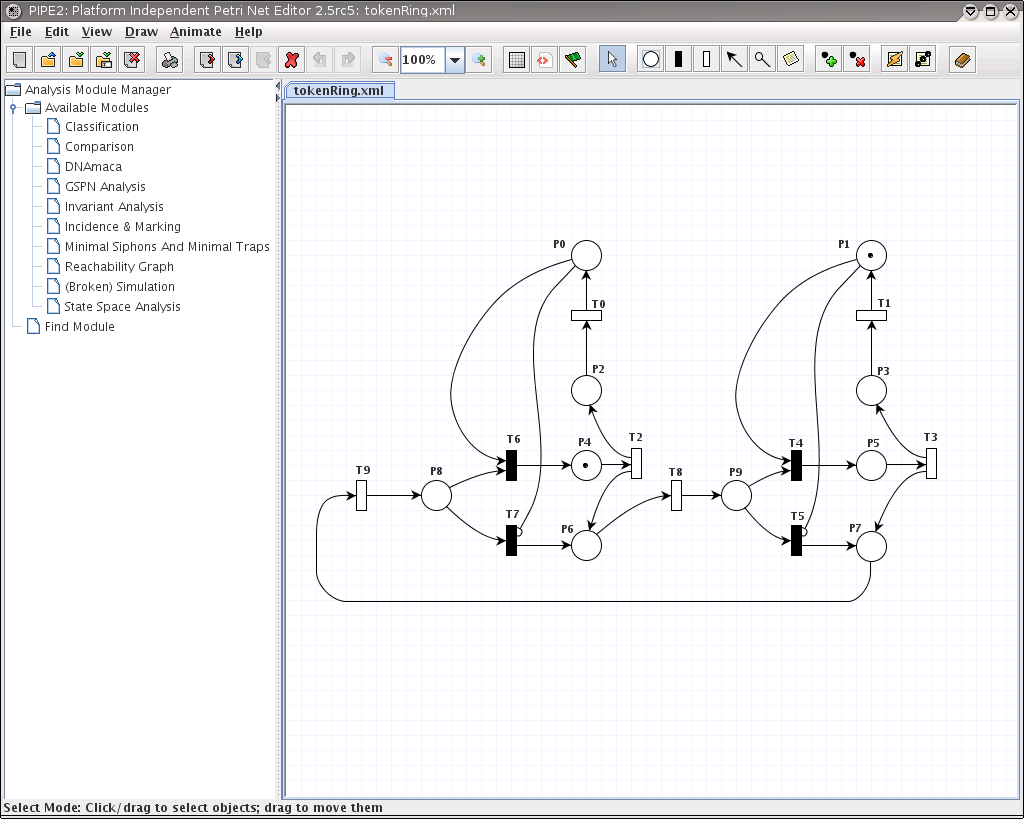
\includegraphics[width=14cm]{image/pipe.png}}
\begin{figure}[!hbt]
\centering
\usebox{\pipeshot}
\caption{PIPE 5 的运行界面} \label{fig:pipeshot}
\end{figure}
